%!TEX ROOT = thesis.tex
\chapter{Framework Overview}
\label{chapter:framework}
\section{Introduction}
To tackle the issues identified through the research questions and literature review, a theoretical framework is first laid out to provide a conceptual schema to break the intricate problem into multiple sub-tasks. Firstly, the overview of the proposed framework used in this work is described in Section \ref{section:framework}. Next, the description of the dataset used is given in Section \ref{section:dataset_used} and finally, this chapter concludes with the experimental methodology applied to obtain the results (presented in Section \ref{sec:expmethodology}).


\section{Framework Overview}
\label{section:framework}
In this section, a high-level overview of the fundamental processes along with the two core components of vehicle semantic attributes extraction and retrieval is provided.
The groundwork described in this work abides by the typical top-down approach used in Intelligent Transportation System (ITS) where the video data is subjected to background subtraction, followed by blob filtering, vehicle detection as well as vehicle tracking, as thoroughly described in \cite{lim2017}.
As the extraction of bounding box is outside the scope of this thesis (see Section \ref{subsec:scope}), the bounding box of the vehicles are assumed to have been obtained prior to the semantic attributes extraction task. Hence, the semantic attribute extraction and video retrieval processes are the central emphasis of this thesis.

In this work, the vehicle colour and vehicle motions were chosen as object-specific semantics to represent events in a car park setting. Additional metadata such as date and time of these event were also extracted as they are crucial elements making up the event timeline. 
These vehicle-specific semantics attribute are then stored in the database.
A retrieval engine was designed to enable users to easily retrieve the stored information. The retrieval engine feature a graphical user interface (GUI) that allow users to enter the queries by drawing the desired trajectory on the search interface and provide other crucial information which would assist in identifying the targeted video sub-sequence or \emph{shot}.


\begin{figure}[hbt!]\centering
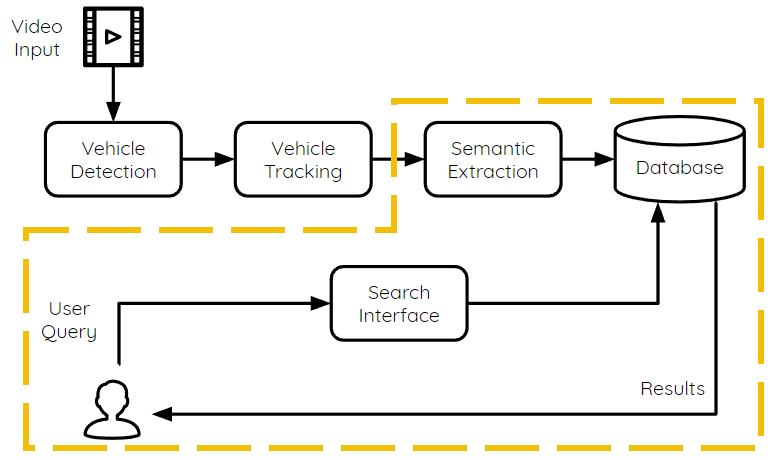
\includegraphics[width=.9\textwidth]{image/new/framework_new.PNG}
\caption{Framework Diagram. Contribution Highlighted in Area Marked with Yellow Dashed Borders.}
\label{fig:framework}
\end{figure}

In this thesis, a framework is suggested and used for the vehicle semantic attribute extraction and vehicle semantic retrieval tasks. The end-to-end framework can be visualised using Figure ~\ref{fig:framework} where the main contribution of this thesis is highlighted with a yellow dashed border.

% \vspace{1em}
% \subsection{Phase 1: LSH-Inspired Semantic Extraction and Retrieval Technique}
% \label{subsec:lsh-intro}
% The first of the two techniques suggested in this thesis is the \textit{LSH-Inspired Semantic Extraction and Retrieval Technique}. Locality-Sensitive Hashing (LSH) as introduced by~\citeA{indyk1998approximate} was originally used for devising main memory algorithms for nearest neighbor search. This technique was later used by~\citeA{kulis2009kernelized} to embed high-dimensional features from images into low-dimensional Hamming space (dimensionality reduction) where items can be efficiently search. 
% Unlike conventional hashing techniques that aims to avoid hash collisions, LSH tries to maximise these hash collisions. When performed on a set of documents, documents with similar properties are mapped and clustered to a similar locality or neighbourhood. This technique excels especially when working with high dimensional data such as video data.
% %However, the exact implementation of LSH is not employed in this work. Instead, 
% We draw inspiration from LSH on how similar ``documents'' can be clustered. %and implemented in this phase. 
% The extracted semantics from each vehicle blobs were clustered into semantic groups consisting of 11 colours and 9 motion clusters. This concept is adopted in the proposed method with the following considerations in mind:
% \begin{enumerate}
%     \item Easing Interpretation \& Access: As the extracted semantics are stored in clusters of similar properties, these semantics can be easily interpreted and retrieved when required.
%     \item Easing Input/Output (I/O) Bottleneck: As the proposed method stores the extracted semantics in a database, I/O bottlenecks are bound to occur when reading and retrieving large quantities of data. Given that semantics of similar properties were clustered together, the retrieval technique only has to search through these identified semantic clusters in an efficient manner instead of the entire database for matching records.
% \end{enumerate}

% TODO: Clarence
% rework on this chapter... explain about chamfer distance, and try to make it link with the previous paragraph since a lot of things doesnt make sense now.
% \vspace{1em}
% \subsection{Semantic Attributes Extraction and Distance-based Retrieval Techniques}




% The second technique suggested in this thesis is the \textit{Chamfer Distance-Inspired Semantic Extraction and Retrieval Technique}.
% Chamfer Distance (CD) is one of the many distance measures %(see Section \ref{section:distancemeasures})
% introduced by mathematicians and researchers. Chamfer Distance, as introduced by~\citeA{barrow1977parametric}, was originally designed to match images by comparing the shapes of two collections of shape fragments.
% However, in this thesis, the use of CD was adapted to suit the research problem of comparing vehicle trajectories' shapes. While the implementation of CD measure in this framework has its advantages, it also comes with certain drawbacks. The considerations taken when designing this technique is as follows:
% \begin{enumerate}
%     \item The use of Chamfer Distance to compare trajectories allows the retrieval technique to search from a wider range. While this comes with additional computational costs which are undesirable, the increased in robustness outweighs the drawbacks. Along with that, effective time and date filtering could potentially reduce the number of records, hence, further reducing the computational cost.
%     \item Effective ranking of results is a desirable characteristic in any retrieval engine. As Chamfer Distance produces a distance score for every pair of trajectories compared, this score can be used to sort the results in an intuitive manner where results of higher similarity or resemblance would appear higher in the ranked retrieval results.
% \end{enumerate}


\section{Dataset}
\label{section:dataset_used}

In view of testing the proposed framework, a new video dataset was gathered as there are limited long-term outdoor car park datasets that are publicly available for research. A stationary cloud-enabled web camera was set up in a room (with a glass window) on the fourth floor of a building facing a relatively large outdoor car park area. Figure \ref{fig:camerasetup} illustrates the location of the camera that was set up to overlook the adjacent car park area. 
%The camera viewpoint is shown in Figure \ref{fig:viewfromcamera}.
%The aforementioned setup was done to mimic a typical camera setup which towers over a piece of outdoor car park lot that is found in the wild.

\begin{figure}[hbt!]\centering
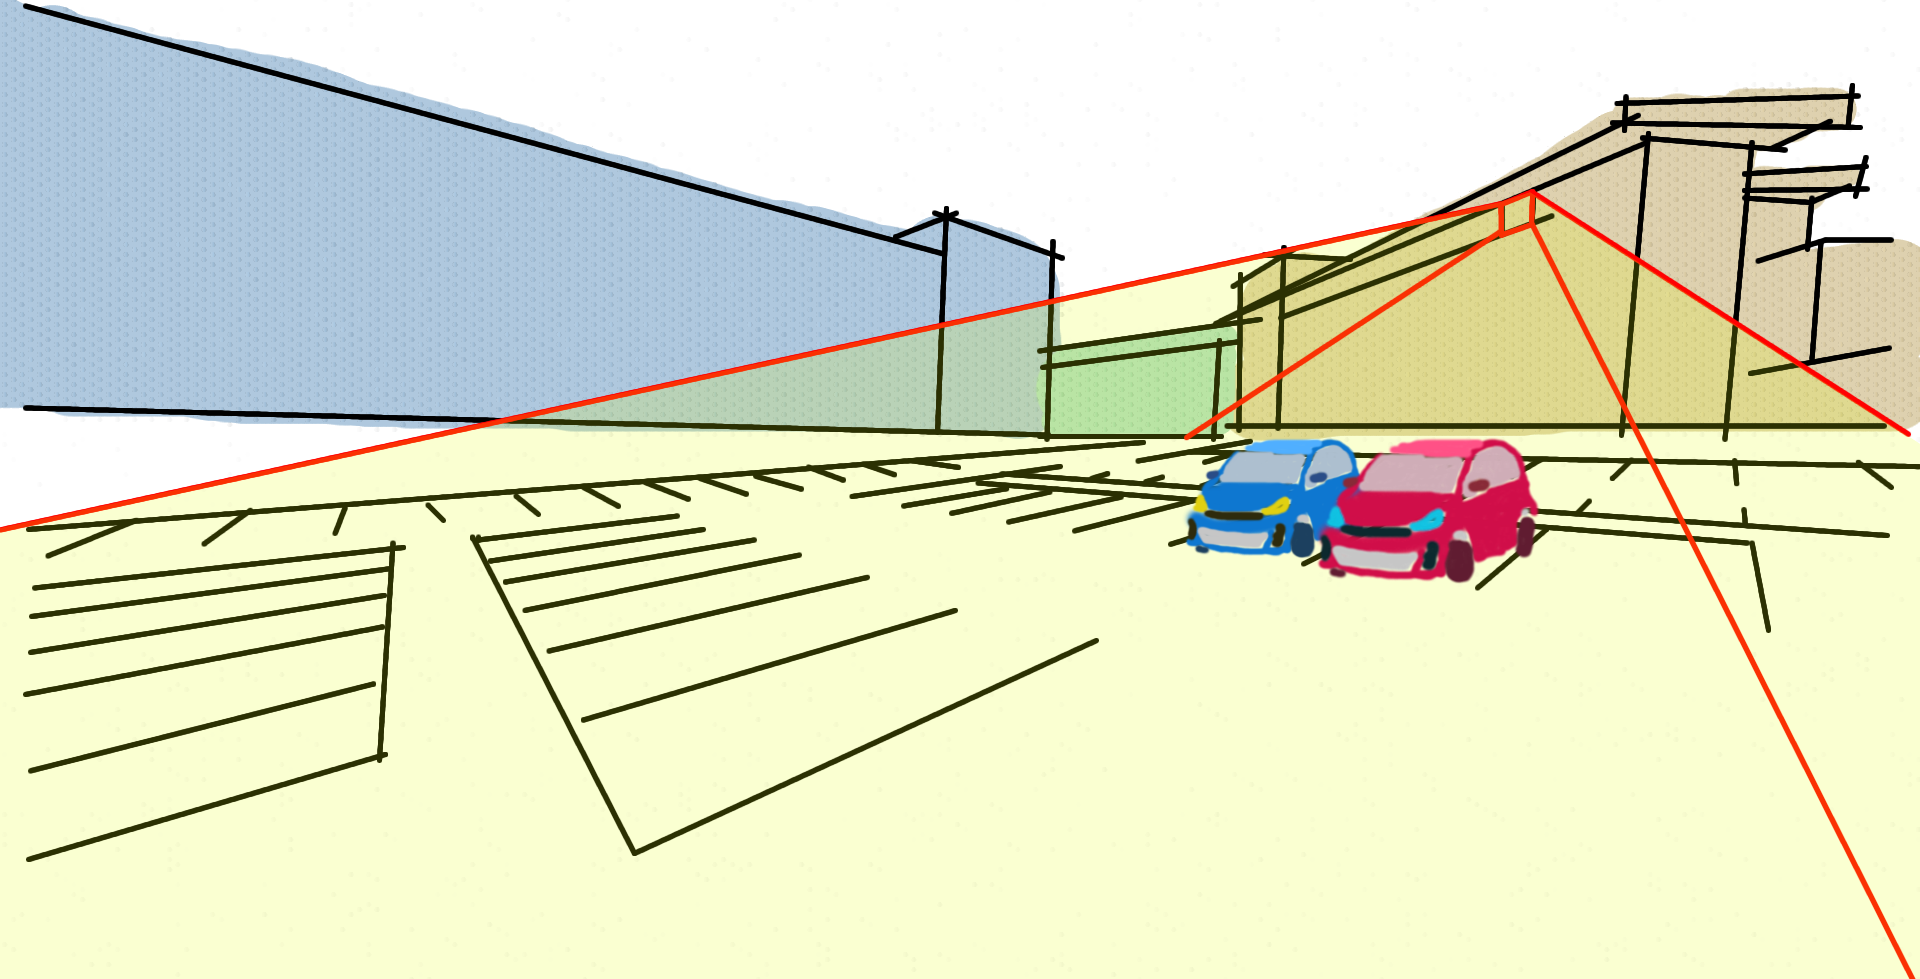
\includegraphics[width=.8\textwidth]{image/new/fcicarpark2.png}
\caption{Camera Setup to Capture the Monitored Outdoor Car Park}
\label{fig:camerasetup}
\end{figure}



Through the camera's web interface, the device was set to record on weekdays from Monday through Friday, starting from 08:30 up until 18:30 in the evening, totalling 10 hours of video recorded each day. As the camera occasionally suffers from recording error, each recorded video clip was set to have a maximum length of 6 minutes to avoid large chunks of missing data. With this setting, a total of 100 videos were obtained at the end of each day. These recorded video clips were stored in a microSD memory card.
At the end of each day, the data was copied over to a server via a script. 

\begin{table}[!bt]\centering
\caption{Details of the Camera Setup used for Data Collection}
\begin{tabular}{|l|l|}
\hline
Camera Model & Dlink DSC-942L        \\
Resolution   & 640$\times$480 pixels \\
Frame rate   & 10 $fps$             \\
Format       & H.264 / MPEG-4 AVC    \\
Naming Convention & $CCYYMMDD\_HHMMSS.mp4$ \\
\hline
\end{tabular}
\end{table}

\begin{figure}[!tb]
  \centering
  \begin{tabular}{cc}
 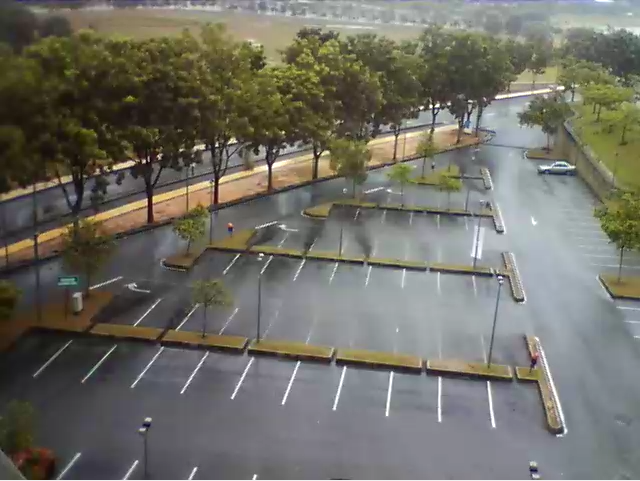
\includegraphics[width=0.4\linewidth]{image/general/rain.PNG} &  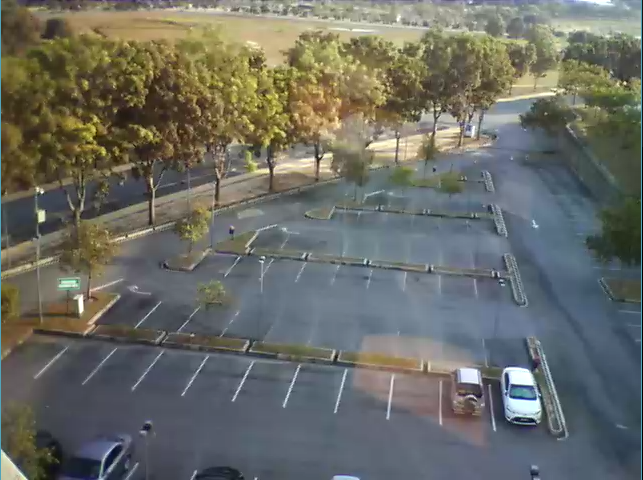
\includegraphics[width=0.4\linewidth]{image/general/reflection.PNG}\\
\begin{tabular}{c}(a) Rainy day with \\ reflective surface\end{tabular} & \begin{tabular}{c}(b) Reflection on the \\car park from the window\end{tabular} \\
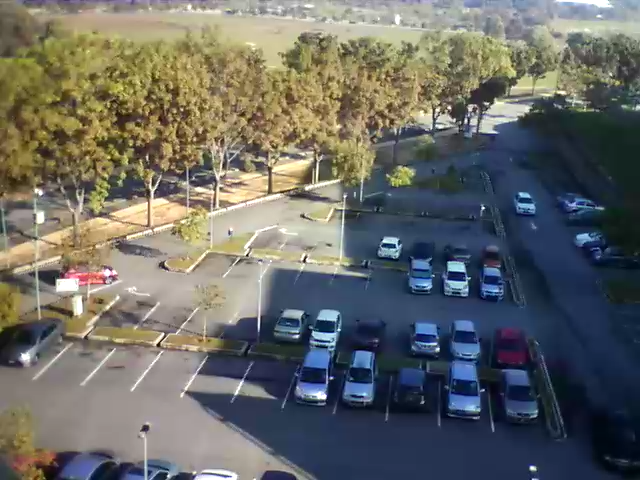
\includegraphics[width=0.4\linewidth]{image/general/shadow.png} &  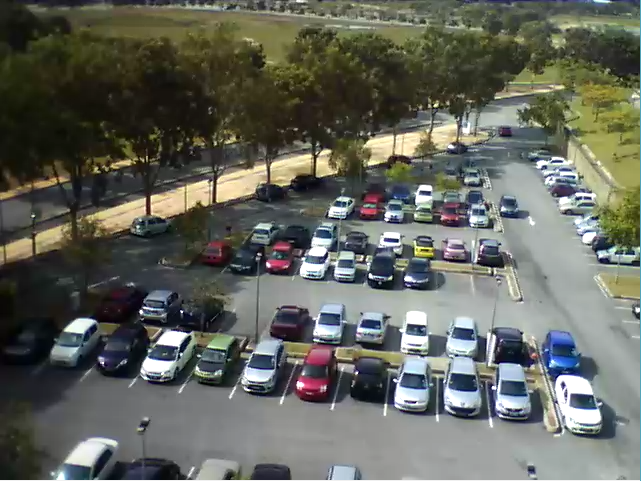
\includegraphics[width=0.4\linewidth]{image/general/shadow2.png}\\
\begin{tabular}{c}(c) Severe shadow over \\ the car park (08:48AM)\end{tabular} & \begin{tabular}{c}(d)  Severe shadow over \\ the car park (04:06PM)\end{tabular}
\end{tabular}
\caption{Challenging Scenarios in the Collected Dataset} \label{fig:weather}
\end{figure}

This data acquisition setup was left unmanned to record data over the course of several months under various natural weather and environmental lighting conditions. The acquisition process captured a diverse set of car park scenes ranging from peak hours with almost a full car park with plenty of vehicles to the less crowded hours of the day. 
%along with the off days. 
% comment: "off days" is colloquial
The setup covers a total of over 45 parking lots excluding parking lots that are too small or occluded (\emph{e.g.} in the last two rows farthest from the camera). Figure \ref{fig:weather} depicts the various challenging weather conditions (rain, glaring sunlight casting shadows) and reflection from the window in front of camera. 
%which were recorded sporadically throughout the dataset.
Since the extraction of bounding boxes of the vehicles is beyond the scope of this thesis, 1 month of bounding box data from the works of \cite{lim2017} was utilized.  

\section{Experimental Methodology}
\label{sec:expmethodology}

This section presents the methodology and the experimental setup to describe how the experiments were performed in this thesis.
In the subsequent chapters, the detailed description of the proposed vehicle semantic attributes extraction algorithm as well as the retrieval technique will be discussed. 

Given that the performance of the proposed method is essential towards end-users, each of the proposed algorithms in the framework is evaluated with the help of volunteers assuming the role as end-users.
A group of six volunteers were tasked to perform a total of 11 queries on the retrieval engine for both the vehicle colour and trajectory semantics.
This approach is unbiased as it provides the volunteers with full control and freedom to perform any kinds of query over the search interface.
The demographic information of the volunteers are as listed in Table \ref{tab:volunteerdemo}.
In order to distinctly evaluate the performance of the proposed method, the evaluation of both the trajectory and colour terms are separated. The separation of both evaluations allow further understanding on how to improve the retrieval engine on various aspects. For further practicality, the evaluation methodology proposes to capture the \emph{relevancy} of the retrieval process through a \emph{user-centric} approach. 
\begin{table}[!ht] 
\centering
\caption {Volunteers Demographic Information}
\label{tab:volunteerdemo}
\begin{tabular}{|c|c|c|c|}
\hline
\textbf{Gender} & \textbf{Age} & \textbf{Education Level} & \textbf{Nationality} \\ \hline
Female          & 21           & University               & Taiwanese            \\ \hline
Male            & 21           & University               & Indian               \\ \hline
Female          & 20           & University               & Thai                 \\ \hline
Male            & 20           & University               & Thai                 \\ \hline
Male            & 20           & University               & Indonesian           \\ \hline
Female          & 19           & University               & Indonesian           \\ \hline
\end{tabular}
\end{table}

Since it is not feasible to fully annotated any large scale data, it is not possible to compute Recall and $F_1$-Score. Instead, the Precision@K along with the normalised Discounted Cumulative Gain (nDCG) metrics were employed as a form of explicit relevance feedback. These evaluation of the metrics will be further elaborated in Section~\ref{sec:retrieval-metrics}.
It is worth noting that the bounding boxes obtained using the vehicle detection and tracking framework proposed by \cite{lim2017} included minor errors. These errors may be propagated to the vehicle semantics extraction and retrieval modules, but they are not overlooked nor discarded during the evaluation process. This is done with the intention to provide an end-to-end assessment of the framework.

First, a group of volunteers (\emph{i.e.} the users) are introduced to the retrieval engine along with its features and how the interface system works. A few sample use cases were demonstrated to the volunteers. 
Next, the volunteers were given full control over the user interface and were allowed to draw any query that they were interested in. They were then tasked to provide feedback by rating each result on a predetermined Semantic Differential Scale of 1 to 5,
also known as the relevance score ($REL$). 
From the scale, 1 represents `Not at all' while 5 can be translated as `Perfectly' encapsulates the query.
The volunteers are given full control to draw the input query $\mathbb{P}$ as to mimic a real world scenario. The volunteers were advised to draw realistic looking trajectories that are mainly on the road areas. As there are no limitations on what could be drawn on the search canvas, it was not feasible to  obtain the ``ground-truth'' annotation for every possible motion within the chosen one month's worth of data. 
Hence, the recall rate could not be viably measured for this retrieval engine. 
The \textit{Precision@K} metric is used to identify the number of retrieved results which are relevant to the user while the \textit{nDCG} metrics is used to measure how well the retrieval engine's results were ranked or sorted for the end users.
For the purpose of computing \textit{Precision@K} metric, the results are first converted into a binary evaluation (True (1) / False (0)).  
During the experiment, results that were ranked with `3' were classified as `True' when using the \textit{Precision@K} metric as these results were somewhat relevant to the query.
The $n$-th relevant results (\emph{i.e.} True (1)) from among all $K$ recalled results contribute to the
\textit{Precision@K} score set out in Equation \ref{eq:p@k}):
\begin{equation}
\label{eq:p@k}
Precision@K =  \frac{\sum_{n=1}^K \delta}{K}
\end{equation}
where 
\begin{equation}
\delta=1, \qquad \text{if} \frac{1}{\Psi}\sum S_{n,\psi} \geq 3
\end{equation}
The overall score for the $n$-th result is averaged over the score decisions $S_{n,\psi}$ made by $\Psi$ number of volunteers.
The retrieved results were intentionally ordered randomly to prevent the volunteers from subconsciously rating a higher $REL$ for results higher in a sorted list.

% comment: is the retrieval results randomly ordered, or ordered based on relevance?
%evaluation for each of the randomly ordered retrieved results.

While \textit{Precision@K} metrics is a commonly used metric in retrieval systems, the main disadvantage of this metric is that the evaluation process is done in a rather coarse manner. 
This is because it only provides a binary evaluation of whether or not a particular result is relevant to the query. On the other hand, the \textit{DCG} metric is able to provide a more granular evaluation of the proposed method as the results are evaluated based on its ordered relevancy rank. Figure~\ref{fig:dcgGain} illustrates the decreasing gain value of each result as the ranking of the
result increases.
The intuition behind the classic Discounted Cumulative Gain (\textit{DCG}) metric~\cite{jarvelin2002cumulated} is that highly relevant results are more useful when it appears higher in rank (hence, a higher gain). This has practical implications; users would not need to go through a large set of results before finding suitable and/or relevant results that the user desires. Likewise, relevant documents which appear lower in the rank should be penalised, hence warranting a discount in its gain.

\begin{figure}[!tb]
\centering
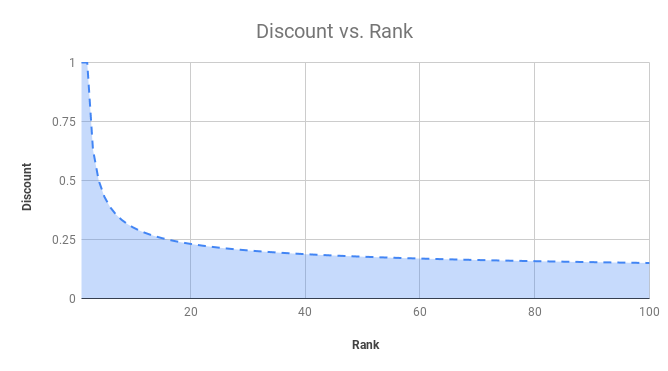
\includegraphics[width=0.9\textwidth]{image/retrievalTwo/discountvsrank.png}
\caption{The Discounted Gain Decreases Exponentially as Rank Increases}
\label{fig:dcgGain}       % Give a unique label
\end{figure}
\begin{equation}
\label{eq:DCGk}
DCG_p = \sum_{p=1}^k\frac{REL_{p}}{\log_2 (\max (p,2))}
\end{equation}
% $DCG@K = \sum_{i=i}^K\frac{REL_{i}}{\log_2 (\max (i,2))}$

Since the Discounted Cumulative Gain metric shown in Equation~\ref{eq:DCGk} produces an unbounded value ([0, $\infty$) range), it is not suitable for use when averaging across multiple independent queries. In order to make use of the \textit{DCG} metric, the normalized version (\textit{nDCG}) shown in Equation~\ref{eq:nDCG} where
the values are now bounded within a [0, 1] range is used instead.
\begin{align}
\label{eq:nDCG}
\textit{nDCG}_k = \frac{DCG_k}{IDCG_k}
\end{align}
$IDCG_P$ is the ideal $DCG$ score at Rank $k$ in the ideal ranking order.


The proposed methods were implemented and evaluated on an Intel i7 machine with 16GB RAM, equipped with a GeForce GTX 1060 GPU. As the main focus of the proposed method revolves around the semantic attribute extraction and retrieval of \textbf{vehicle colour} and \textbf{vehicle trajectory}. Both of these components were assessed and evaluated individually to better understand the performance, effectiveness and to analyse the weaknesses of the proposed methods.

% As a result, two different phases were introduced to enhance the performance based on the 
% % comment: what is "intel" ?
% %obtained intel and 
% gaps which were identified via experimental results. This also allows us to gain a deeper understanding of the proposed method along with opportunities for future improvements.
% Likewise, the experimental methodology can be divided into two phases, as discussed in the following sections.
% %Two retrieval techniques were designed and implemented in this work, the objective of the first retrieval engine was to build a prototype for the evaluation of its current performance and to identify gaps to be improved. This process allowed the author to return to the drawing board and reevaluate the algorithms, metrics and evaluation process performed.


% \vspace{1em}
% \subsection{Phase 1: LSH-Inspired Semantic Extraction and Retrieval Technique (Prototyping)}
% While the collected dataset comprised of several months of data, only two days of data (20 hours) were used for the evaluation of \versionOneRet. Several annotators were tasked to manually annotate the data. Upon completing the annotation process, the annotators would then cross-check annotations from other annotators to verify the consistency of the annotations.
% In the process, the annotators were asked to arrive at a consensus for specific annotations that did not tally. The annotators were also asked to record the following events:
% 1) Number of vehicle of each colour category (11 categories, see Table~\ref{table:colorshex}), and 2) Number of vehicles performing designated motion test cases (denoted as $TQ1$ \& $TQ2$, see Figure \ref{fig:versionOneInterface}).
% The availability of fully annotated data allows the performance of the proposed method to be evaluated using the metrics such as Accuracy, Recall and $F_1$-Score.

% the entire annotation process took a significant amount of work despite only performing on two days of data. Since one month of data was set aside for the evaluation of the \versionTwoRet, an alternative experimental methodology was applied.
% Typical with the evaluation of most large-scale retrieval engines~\cite{jermsurawong2012car, zhang2013mining, castanon2016retrieval, ren2018learning}, 
% % comment: removed. confusing.
% %of all intents and purposes, 
% it is not feasible to annotate a huge amount of ground truth labels manually as it is both %takes an enormous effort which is 
% time-consuming and costly. 
% Hence in \textbf{Phase 2}, the semantics from one month of data were extracted, retrieved and evaluated without the manual annotations of any events.

% As the final output of this proposed method is an end-user facing retrieval system, the evaluation process took on an empirical user study approach. 
